\documentclass{article}
\usepackage{luatextra}
\usepackage{polyglossia}
\usepackage{ulem}
\usepackage{framed}
\usepackage{color}
\usepackage{geometry}
\usepackage{amsmath}
\usepackage{unicode-math}
\usepackage[hidelinks]{hyperref}
\usepackage{latexsym}
\usepackage{pdflscape}
\usepackage{pdfpages}
\usepackage{enumitem}
\usepackage{titlesec}
\usepackage{lastpage}
\usepackage{fancyhdr}
\usepackage{titlesec}
\usepackage{listings}
\usepackage{graphicx}
\usepackage{float}
\usepackage{pdfpages}

\usepackage{ifluatex}
\ifluatex
  \usepackage{pdftexcmds}
  \makeatletter
  \let\pdfstrcmp\pdf@strcmp
  \let\pdffilemoddate\pdf@filemoddate
  \makeatother
\fi
\usepackage{svg}

\setmathfont{xits-math.otf}

\setmainlanguage{french}
\selectlanguage{french}
%%\setmainfont{Latin Modern Roman}
\setmainfont{Roboto}

\geometry{margin={1in,1in}}

\setlist{nosep} %% No space between lists' items

\pagestyle{fancy}
\fancyhead[R]{}

%% <current page>/<total pages> footer
\cfoot{\thepage/\pageref{LastPage}}

\newcommand\image[2]{
\directlua{
local image = img.scan({filename = "#1"})

image.height = image.height * #2
image.width  = image.width  * #2

node.write(img.node(image))
}
}


%%%%%%%%%%%%%%%%%%%%%%%%%%%%%%%%%%%%%%%%%%
%% \subsubsubsection command definition %%
%%%%%%%%%%%%%%%%%%%%%%%%%%%%%%%%%%%%%%%%%%


\titleclass{\subsubsubsection}{straight}[\subsection]

\newcounter{subsubsubsection}[subsubsection]
\renewcommand\thesubsubsubsection{\thesubsubsection.\arabic{subsubsubsection}}
\renewcommand\theparagraph{\thesubsubsubsection.\arabic{paragraph}} % optional; useful if paragraphs are to be numbered

\titleformat{\subsubsubsection}
  {\normalfont\normalsize\bfseries}{\thesubsubsubsection}{1em}{}
\titlespacing*{\subsubsubsection}
{0pt}{3.25ex plus 1ex minus .2ex}{1.5ex plus .2ex}

\makeatletter
\renewcommand\paragraph{\@startsection{paragraph}{5}{\z@}%
  {3.25ex \@plus1ex \@minus.2ex}%
  {-1em}%
  {\normalfont\normalsize\bfseries}}
\renewcommand\subparagraph{\@startsection{subparagraph}{6}{\parindent}%
  {3.25ex \@plus1ex \@minus .2ex}%
  {-1em}%
  {\normalfont\normalsize\bfseries}}
\def\toclevel@subsubsubsection{4}
\def\toclevel@paragraph{5}
\def\toclevel@paragraph{6}
\def\l@subsubsubsection{\@dottedtocline{4}{7em}{4em}}
\def\l@paragraph{\@dottedtocline{5}{10em}{5em}}
\def\l@subparagraph{\@dottedtocline{6}{14em}{6em}}
\makeatother

\setcounter{secnumdepth}{4}
\setcounter{tocdepth}{4}

%%%%%%%%%%%%%%%%%%%%%%%%%%%%%%%%%%%%%%%%%%
%% end \subsubsubsection definition     %%
%%%%%%%%%%%%%%%%%%%%%%%%%%%%%%%%%%%%%%%%%%


\titlespacing*{\section}{0pt}{0.7\baselineskip}{0.7\baselineskip}

\title{Projet Principe d'éxécution des programmes}
%\subtitle{Meow}
\author{NassimBounouas, piernov}
\date{\today}

\begin{document}
\lstset{xleftmargin=.25in}

\maketitle
\textcolor{blue}{\url{https://github.com/NassimBounouas/Stage_SI3_PeP}}
\tableofcontents

\newpage

\section{Présentation du projet}
\subsection{Le microprocesseur ARM Cortex-M0}
	La famille des ARM Cortex M regroupe des processeurs 32 bits. Ils peuvent être utilisés comme microprocesseur ou microcontrôleur. On les retrouve dans diverses applications : Arduino Due,  Machine à laver, distributeur de boissons...  Les cortex M vise en majorité le marché de l'embarqué.

	Le but de ce projet est de simuler le comportement d'un cortex M0 au moyen d'un logiciel de simulation électronique (logisim). L'idée est ici d'obtenir un système ayant un comportement similaire à un Cortex M0 et non une copie conforme du fait de la complexité d'un processeur réel.

\subsection{Assembleur}

	Le code binaire a exécuter est obtenu par l'assemblage d'instructions issus du jeu d'instructions ARMv7 (contre un jeu ARMv6 dans le cortex M0 réel).

\subsubsection{Syntaxe}
Syntaxe UAL\\
S: màj des drapeaux\\
<c>: condition\\
Rd: registre destination\\
<imm?>: immédiat\\
SP: registre de pointeur de pile en mémoire\\
opcode: code de l'instruction, peut occuper jusqu'à la taille indiquée\\
\[\]: argument optionnel\\

Example:
\begin{lstlisting}
.LBBH:                                
	ldr	r0, [sp, #4]
	ldr	r1, [sp, #28]
	cmp	r0, r1
	bge	.LBBK
	b	.LBBI
.LBBI:                                
	ldr	r0, [sp, #20]
	movs	r1, #1
	ands	r0, r1
	str	r0, [sp, #36]
	ldr	r0, [sp, #32]
	subs	r0, r1, r0
	str	r0, [sp, #32]
	ldr	r0, [sp, #32]
	ldr	r1, [sp, #36]
	lsls	r1, r1, #1
	adds	r0, r0, r1
	str	r0, [sp, #52]
	ldr	r0, [sp, #20]
	asrs	r0, r0, #1
	str	r0, [sp, #20]
	b	.LBBJ
\end{lstlisting}

\section{Jeu d'instructions (Instruction Set Architecture)}
\label{sec:ISA}

Toutes les informations présentes dans cette section proviennent directement du manuel de référence de l'achitecture ARMv7-M (\textit{ARM v7-M Architecture Reference Manual}). Elles ont été traduites et réorganisées pour en faciliter la lecture.
En cas de doute, ou pour en savoir plus, les pages du manuel sont indiquées entre parenthèses.

\subsection{Instructions à implémenter}

\textbf{Binaire:}\\

\begin{tabular}{| c c c c c c c c c c c c c c c c |}
\hline
15 & 14 & 13 & 12 & 11 & 10 & \multicolumn{1}{|c}{9} & 8 & 7 & 6 & 5 & 4 & 3 & 2 & 1 & 0 \\
\hline
\multicolumn{6}{|c}{opcode} & \multicolumn{10}{|c|}{} \\
\hline
\end{tabular}


\subsubsection{Shift, add, sub, mov}
\label{subsubsec:ShiftAddSubMov}

\textbf{Binaire:}\\

\begin{tabular}{| c c c c c c c c c c c c c c c c |}
\hline
15 & 14 & \multicolumn{1}{|c}{13} & 12 & 11 & 10 & 9 & \multicolumn{1}{|c}{8} & 7 & 6 & 5 & 4 & 3 & 2 & 1 & 0 \\
\hline
0 & 0 & \multicolumn{5}{|c}{opcode} & \multicolumn{9}{|c|}{} \\
\hline
\end{tabular}


\subsubsubsection{LSL (immediate): Logical Shift Left (p. 298)}

\textbf{Description: }

Décale le contenu du registre \texttt{Rm} vers la gauche d'un nombre de bits donné par l'immédiat \texttt{imm5}, écrit le résultat dans le registre \texttt{Rd}.\\
Des zéros sont insérés à droite.\\
Les drapeaux suivants sont mis à jour:\\
\texttt{N = 1} si \texttt{résultat < 0}, \texttt{N = 0} sinon.\\                                      
\texttt{Z = 1} si \texttt{résultat = 0}, \texttt{Z = 0} sinon.\\
\texttt{C = Rm<0 - shift>} avec shift le nombre de décalage. Autrement dit, \texttt{C} est égal au dernier bit sortant.\\

\textbf{Assembleur:} T1

\begin{lstlisting}
LSLS <Rd>,<Rm>,#<imm5>
\end{lstlisting}

\textbf{Binaire:}\\

\begin{tabular}{| c c c c c c c c c c c c c c c c |}
\hline
15 & 14 & 13 & \multicolumn{1}{|c}{12} & 11 & \multicolumn{1}{|c}{10} & 9 & 8 & 7 & 6 & \multicolumn{1}{|c}{5} & 4 & 3 & \multicolumn{1}{|c}{2} & 1 & 0 \\
\hline
0 & 0 & 0 & \multicolumn{1}{|c}{0} & 0 & \multicolumn{5}{|c|}{imm5} & \multicolumn{3}{|c|}{Rm} & \multicolumn{3}{|c|}{Rd} \\
\hline
\end{tabular}

\subsubsubsection{LSR (immediate): Logical Shift Right (p. 302)}

\textbf{Description: }

Décale le contenu du registre \texttt{Rm} vers la droite d'un nombre de bits donné par l'immédiat \texttt{imm5}, écrit le résultat dans le registre \texttt{Rd}.\\
Des zéros sont insérés à gauche.\\
Les drapeaux suivants sont mis à jour:\\
\texttt{N = 1} si \texttt{résultat < 0}, \texttt{N = 0} sinon.\\
\texttt{Z = 1} si \texttt{résultat = 0}, \texttt{Z = 0} sinon.\\
\texttt{C = Rm<shift - 1>} avec shift le nombre de décalage. Autrement dit, \texttt{C} est égal au dernier bit sortant.\\

\textbf{Assembleur:} T1

\begin{lstlisting}
LSRS <Rd>,<Rm>,#<imm5>
\end{lstlisting}

\textbf{Binaire:}\\

\begin{tabular}{| c c c c c c c c c c c c c c c c |}
\hline
15 & 14 & 13 & \multicolumn{1}{|c}{12} & 11 & \multicolumn{1}{|c}{10} & 9 & 8 & 7 & 6 & \multicolumn{1}{|c}{5} & 4 & 3 & \multicolumn{1}{|c}{2} & 1 & 0 \\
\hline   
0 & 0 & 0 & \multicolumn{1}{|c}{0} & 1 & \multicolumn{5}{|c|}{imm5} & \multicolumn{3}{|c|}{Rm} & \multicolumn{3}{|c|}{Rd} \\
\hline
\end{tabular}


\subsubsubsection{ASR (immediate): Arithmetic Shift Right (p. 203)}

\textbf{Description: }

Décale le contenu du registre \texttt{Rm} vers la droite d'un nombre de bits donné par l'immédiat \texttt{imm5}, écrit le résultat dans le registre \texttt{Rd}.\\
Le bit de signe de \texttt{Rm} est ré-inséré à gauche.\\
Les drapeaux suivants sont mis à jour:\\
\texttt{N = 1} si \texttt{résultat < 0}, \texttt{N = 0} sinon.\\
\texttt{Z = 1} si \texttt{résultat = 0}, \texttt{Z = 0} sinon.\\
\texttt{C = Rm<shift - 1>} avec shift le nombre de décalage. Autrement dit, \texttt{C} est égal au dernier bit sortant.\\

\textbf{Assembleur:} T1

\begin{lstlisting}
ASRS <Rd>,<Rm>,#<imm5>
\end{lstlisting}

\textbf{Binaire:}\\

\begin{tabular}{| c c c c c c c c c c c c c c c c |}
\hline
15 & 14 & 13 & \multicolumn{1}{|c}{12} & 11 & \multicolumn{1}{|c}{10} & 9 & 8 & 7 & 6 & \multicolumn{1}{|c}{5} & 4 & 3 & \multicolumn{1}{|c}{2} & 1 & 0 \\
\hline   
0 & 0 & 0 & \multicolumn{1}{|c}{1} & 0 & \multicolumn{5}{|c|}{imm5} & \multicolumn{3}{|c|}{Rm} & \multicolumn{3}{|c|}{Rd} \\
\hline
\end{tabular}


\subsubsubsection{ADD (register): Add register (p. 191)}

\textbf{Description: }

Ajoute le contenu du registre \texttt{Rn} au contenu du registre \texttt{Rm}, écrit le résultat dans le registre \texttt{Rd}.\\
Les drapeaux suivants sont mis à jour:\\
\texttt{N = 1} si \texttt{résultat < 0}, \texttt{N = 0} sinon.\\
\texttt{Z = 1} si \texttt{résultat = 0}, \texttt{Z = 0} sinon.\\
\texttt{C = 1} en cas de dépassement de capacité lors d'une opération non signée.\\
\texttt{V = 1} en cas de dépassement de capacité lors d'une opération signée.\\

\textbf{Assembleur:} T1

\begin{lstlisting}
ADDS <Rd>,<Rn>,<Rm>
\end{lstlisting}

\textbf{Binaire:}\\

\begin{tabular}{| c c c c c c c c c c c c c c c c |}
\hline
15 & 14 & 13 & \multicolumn{1}{|c}{12} & 11 & \multicolumn{1}{|c}{10} & \multicolumn{1}{|c}{9} & \multicolumn{1}{|c}{8} & 7 & 6 & \multicolumn{1}{|c}{5} & 4 & 3 & \multicolumn{1}{|c}{2} & 1 & 0 \\
\hline   
0 & 0 & 0 & \multicolumn{1}{|c}{1} & 1 &  \multicolumn{1}{|c}{0} & \multicolumn{1}{|c}{0} & \multicolumn{3}{|c|}{Rm} & \multicolumn{3}{|c|}{Rn} & \multicolumn{3}{|c|}{Rd} \\
\hline
\end{tabular}


\subsubsubsection{SUB (register): Substract register (p. 450)}

\textbf{Description: }
Soustrait le contenu du registre \texttt{Rm} au contenu du registre \texttt{Rn}, écrit le résultat dans le registre \texttt{Rd}.\\
Les drapeaux suivants sont mis à jour:\\
\texttt{N = 1} si \texttt{résultat < 0}, \texttt{N = 0} sinon.\\
\texttt{Z = 1} si \texttt{résultat = 0}, \texttt{Z = 0} sinon.\\
\texttt{C = 1} en cas de dépassement de capacité lors d'une opération non signée.\\    
\texttt{V = 1} en cas de dépassement de capacité lors d'une opération signée.\\

\textbf{Assembleur:} T1

\begin{lstlisting}
SUBS <Rd>,<Rn>,<Rm>
\end{lstlisting}

\textbf{Binaire:}\\

\begin{tabular}{| c c c c c c c c c c c c c c c c |}
\hline
15 & 14 & 13 & \multicolumn{1}{|c}{12} & 11 & \multicolumn{1}{|c}{10} & \multicolumn{1}{|c}{9} & \multicolumn{1}{|c}{8} & 7 & 6 & \multicolumn{1}{|c}{5} & 4 & 3 & \multicolumn{1}{|c}{2} & 1 & 0 \\
\hline   
0 & 0 & 0 & \multicolumn{1}{|c}{1} & 1 &  \multicolumn{1}{|c}{0} & \multicolumn{1}{|c}{1} & \multicolumn{3}{|c|}{Rm} & \multicolumn{3}{|c|}{Rn} & \multicolumn{3}{|c|}{Rd} \\
\hline
\end{tabular}


\subsubsubsection{ADD (immediate): Add 3-bit immediate (p. 189)}

\textbf{Description: }

Ajoute l'immédiat \texttt{Imm3} au contenu du registre \texttt{Rn}, écrit le résultat dans le registre \texttt{Rd}.\\
Les drapeaux suivants sont mis à jour:\\
\texttt{N = 1} si \texttt{résultat < 0}, \texttt{N = 0} sinon.\\
\texttt{Z = 1} si \texttt{résultat = 0}, \texttt{Z = 0} sinon.\\
\texttt{C = 1} en cas de dépassement de capacité lors d'une opération non signée.\\    
\texttt{V = 1} en cas de dépassement de capacité lors d'une opération signée.\\

\textbf{Assembleur:} T1

\begin{lstlisting}
ADDS <Rd>,<Rn>,<#imm3>
\end{lstlisting}

\textbf{Binaire:}\\

\begin{tabular}{| c c c c c c c c c c c c c c c c |}
\hline
15 & 14 & 13 & \multicolumn{1}{|c}{12} & 11 & \multicolumn{1}{|c}{10} & \multicolumn{1}{|c}{9} & \multicolumn{1}{|c}{8} & 7 & 6 & \multicolumn{1}{|c}{5} & 4 & 3 & \multicolumn{1}{|c}{2} & 1 & 0 \\
\hline   
0 & 0 & 0 & \multicolumn{1}{|c}{1} & 1 &  \multicolumn{1}{|c}{1} & \multicolumn{1}{|c}{0} & \multicolumn{3}{|c|}{Imm3} & \multicolumn{3}{|c|}{Rn} & \multicolumn{3}{|c|}{Rd} \\
\hline
\end{tabular}


\subsubsubsection{SUB (immediate): Subtract 3-bit immediate (p. 448)}

\textbf{Description: }

Soustrait l'immédiat \texttt{Imm3} au contenu du registre \texttt{Rn}, écrit le résultat dans le registre \texttt{Rd}.\\
Les drapeaux suivants sont mis à jour:\\
\texttt{N = 1} si \texttt{résultat < 0}, \texttt{N = 0} sinon.\\
\texttt{Z = 1} si \texttt{résultat = 0}, \texttt{Z = 0} sinon.\\
\texttt{C = 1} en cas de dépassement de capacité lors d'une opération non signée.\\    
\texttt{V = 1} en cas de dépassement de capacité lors d'une opération signée.\\

\textbf{Assembleur:} T1

\begin{lstlisting}
SUBS <Rd>,<Rn>,#<imm3>
\end{lstlisting}

\textbf{Binaire:}\\

\begin{tabular}{| c c c c c c c c c c c c c c c c |}
\hline
15 & 14 & 13 & \multicolumn{1}{|c}{12} & 11 & \multicolumn{1}{|c}{10} & \multicolumn{1}{|c}{9} & \multicolumn{1}{|c}{8} & 7 & 6 & \multicolumn{1}{|c}{5} & 4 & 3 & \multicolumn{1}{|c}{2} & 1 & 0 \\
\hline   
0 & 0 & 0 & \multicolumn{1}{|c}{1} & 1 &  \multicolumn{1}{|c}{1} & \multicolumn{1}{|c}{1} & \multicolumn{3}{|c|}{Imm3} & \multicolumn{3}{|c|}{Rn} & \multicolumn{3}{|c|}{Rd} \\
\hline
\end{tabular}


\subsubsubsection{MOV (immediate): Move (p. 312)}

\textbf{Description: }

Écrit l'immédiat \texttt{imm8} dans le registre \texttt{Rd}.\\
Les drapeaux suivants sont mis à jour:\\
\texttt{N = 1} si \texttt{résultat < 0}, \texttt{N = 0} sinon.\\
\texttt{Z = 1} si \texttt{résultat = 0}, \texttt{Z = 0} sinon.\\

\textbf{Assembleur:} T1

\begin{lstlisting}
MOVS <Rd>,#<imm8>
\end{lstlisting}

\textbf{Binaire:}\\

\begin{tabular}{| c c c c c c c c c c c c c c c c |}
\hline
15 & 14 & 13 & \multicolumn{1}{|c}{12} & 11 & \multicolumn{1}{|c}{10} & 9 & 8 & \multicolumn{1}{|c}{7} & 6 & 5 & 4 & 3 & 2 & 1 & 0 \\
\hline
0 & 0 & 1 & \multicolumn{1}{|c}{0} & 0 & \multicolumn{3}{|c|}{Rd} & \multicolumn{8}{|c|}{imm8} \\
\hline
\end{tabular}


\subsubsection{Data processing}
\label{subsubsec:DataProc}

\textbf{Binaire:}\\

\begin{tabular}{| c c c c c c c c c c c c c c c c |}
\hline
15 & 14 & 13 & 12 & 11 & 10 & \multicolumn{1}{|c}{9} & 8 & 7 & 6 & \multicolumn{1}{|c}{5} & 4 & 3 & 2 & 1 & 0 \\
\hline
0 & 1 & 0 & 0 & 0 & 0 & \multicolumn{4}{|c}{opcode} & \multicolumn{6}{|c|}{} \\
\hline
\end{tabular}

\subsubsubsection{AND (register): Bitwise AND (p. 201)}

\textbf{Description: }

Effectue un ET binaire entre le contenu du registre \texttt{Rdn} et le contenu du registre \texttt{Rm}, écrit le résultat dans le registre \texttt{Rdn}.\\
Les drapeaux suivants sont mis à jour:\\
\texttt{N = 1} si \texttt{résultat < 0}, \texttt{N = 0} sinon.\\
\texttt{Z = 1} si \texttt{résultat = 0}, \texttt{Z = 0} sinon.\\
\texttt{C = 0}\\

\textbf{Assembleur:} T1

\begin{lstlisting}
ANDS <Rdn>,<Rm>
\end{lstlisting}

\textbf{Binaire:}\\

\begin{tabular}{| c c c c c c c c c c c c c c c c |}
\hline
15 & 14 & 13 & 12 & 11 & 10 & \multicolumn{1}{|c}{9} & 8 & 7 & 6 & \multicolumn{1}{|c}{5} & 4 & 3 & \multicolumn{1}{|c}{2} & 1 & 0 \\
\hline
0 & 1 & 0 & 0 & 0 & 0 & \multicolumn{1}{|c}{0} & 0 & 0 & 0 & \multicolumn{3}{|c}{Rm} & \multicolumn{3}{|c|}{Rdn} \\
\hline
\end{tabular}


\subsubsubsection{EOR (register): Exclusive OR (p. 239)}

\textbf{Description: }

Effectue un OU exclusif binaire entre le contenu du registre \texttt{Rdn} et le contenu du registre \texttt{Rm}, écrit le résultat dans le registre \texttt{Rdn}.\\
Les drapeaux suivants sont mis à jour:\\
\texttt{N = 1} si \texttt{résultat < 0}, \texttt{N = 0} sinon.\\                                                                  
\texttt{Z = 1} si \texttt{résultat = 0}, \texttt{Z = 0} sinon.\\
\texttt{C = 0}\\

\textbf{Assembleur:} T1

\begin{lstlisting}
EORS <Rdn>,<Rm>
\end{lstlisting}

\textbf{Binaire:}\\

\begin{tabular}{| c c c c c c c c c c c c c c c c |}
\hline
15 & 14 & 13 & 12 & 11 & 10 & \multicolumn{1}{|c}{9} & 8 & 7 & 6 & \multicolumn{1}{|c}{5} & 4 & 3 & \multicolumn{1}{|c}{2} & 1 & 0 \\
\hline
0 & 1 & 0 & 0 & 0 & 0 & \multicolumn{1}{|c}{0} & 0 & 0 & 1 & \multicolumn{3}{|c}{Rm} & \multicolumn{3}{|c|}{Rdn} \\
\hline
\end{tabular}


\subsubsubsection{LSL (register): Logical Shift Left (p. 300)}

\textbf{Description: }

Décale le contenu du registre \texttt{Rdn} vers la gauche d'un nombre de bits donné par l'octet inférieur du registre \texttt{Rm}, écrit le résultat dans le registre \texttt{Rdn}.\\
Des zéros sont insérés à droite.\\
Les drapeaux suivants sont mis à jour:\\
\texttt{N = 1} si \texttt{résultat < 0}, \texttt{N = 0} sinon.\\
\texttt{Z = 1} si \texttt{résultat = 0}, \texttt{Z = 0} sinon.\\
\texttt{C = Rn<0 - shift>} avec shift le nombre de décalage. Autrement dit, \texttt{C} est égal au dernier bit sortant.\\

\textbf{Assembleur:} T1

\begin{lstlisting}
LSLS <Rdn>,<Rm>
\end{lstlisting}

\textbf{Binaire:}\\

\begin{tabular}{| c c c c c c c c c c c c c c c c |}
\hline
15 & 14 & 13 & 12 & 11 & 10 & \multicolumn{1}{|c}{9} & 8 & 7 & 6 & \multicolumn{1}{|c}{5} & 4 & 3 & \multicolumn{1}{|c}{2} & 1 & 0 \\
\hline
0 & 1 & 0 & 0 & 0 & 0 & \multicolumn{1}{|c}{0} & 0 & 1 & 0 & \multicolumn{3}{|c}{Rm} & \multicolumn{3}{|c|}{Rdn} \\
\hline
\end{tabular}



\subsubsubsection{LSR (register): Logical Shift Right (p. 304)}

\textbf{Description: }

Décale le contenu du registre \texttt{Rdn} vers la droite d'un nombre de bits donné par l'octet inférieur du registre \texttt{Rm}, écrit le résultat dans le registre \texttt{Rdn}.\\
Des zéros sont insérés à gauche.\\
Les drapeaux suivants sont mis à jour:\\
\texttt{N = 1} si \texttt{résultat < 0}, \texttt{N = 0} sinon.\\
\texttt{Z = 1} si \texttt{résultat = 0}, \texttt{Z = 0} sinon.\\
\texttt{C = Rn<shift - 1>} avec shift le nombre de décalage. Autrement dit, \texttt{C} est égal au dernier bit sortant.\\

\textbf{Assembleur:} T1

\begin{lstlisting}
LSRS <Rdn>,<Rm>
\end{lstlisting}

\textbf{Binaire:}\\

\begin{tabular}{| c c c c c c c c c c c c c c c c |}
\hline
15 & 14 & 13 & 12 & 11 & 10 & \multicolumn{1}{|c}{9} & 8 & 7 & 6 & \multicolumn{1}{|c}{5} & 4 & 3 & \multicolumn{1}{|c}{2} & 1 & 0 \\
\hline
0 & 1 & 0 & 0 & 0 & 0 & \multicolumn{1}{|c}{0} & 0 & 1 & 1 & \multicolumn{3}{|c}{Rm} & \multicolumn{3}{|c|}{Rdn} \\
\hline
\end{tabular}


\subsubsubsection{ASR (register): Arithmetic Shift Right (p. 205)}

\textbf{Description: }

Décale le contenu du registre \texttt{Rdn} vers la droite d'un nombre de bits donné par l'octet inférieur du registre \texttt{Rm}, écrit le résultat dans le registre \texttt{Rdn}.\\
Le bit de signe de \texttt{Rdn} est ré-inséré à gauche.\\
Les drapeaux suivants sont mis à jour:\\
\texttt{N = 1} si \texttt{résultat < 0}, \texttt{N = 0} sinon.\\
\texttt{Z = 1} si \texttt{résultat = 0}, \texttt{Z = 0} sinon.\\
\texttt{C = Rn<shift - 1>} avec shift le nombre de décalage. Autrement dit, \texttt{C} est égal au dernier bit sortant.\\

\textbf{Assembleur:} T1

\begin{lstlisting}
ASRS <Rdn>,<Rm>
\end{lstlisting}

\textbf{Binaire:}\\

\begin{tabular}{| c c c c c c c c c c c c c c c c |}
\hline
15 & 14 & 13 & 12 & 11 & 10 & \multicolumn{1}{|c}{9} & 8 & 7 & 6 & \multicolumn{1}{|c}{5} & 4 & 3 & \multicolumn{1}{|c}{2} & 1 & 0 \\
\hline
0 & 1 & 0 & 0 & 0 & 0 & \multicolumn{1}{|c}{0} & 1 & 0 & 0 & \multicolumn{3}{|c}{Rm} & \multicolumn{3}{|c|}{Rdn} \\
\hline
\end{tabular}


\subsubsubsection{ADC (register): Add with Carry (p. 187)}

\textbf{Description: }

Ajoute le contenu du registre \texttt{Rm} et le drapeau de retenu au contenu du registre \texttt{Rdn}, écrit le résultat dans le registre \texttt{Rdn}.\\
Les drapeaux suivants sont mis à jour:\\
\texttt{N = 1} si \texttt{résultat < 0}, \texttt{N = 0} sinon.\\
\texttt{Z = 1} si \texttt{résultat = 0}, \texttt{Z = 0} sinon.\\
\texttt{C = 1} en cas de dépassement de capacité lors d'une opération non signée.\\
\texttt{V = 1} en cas de dépassement de capacité lors d'une opération signée.\\

\textbf{Assembleur:} T1

\begin{lstlisting}
ADCS <Rdn>,<Rm>
\end{lstlisting}

\textbf{Binaire:}\\

\begin{tabular}{| c c c c c c c c c c c c c c c c |}
\hline
15 & 14 & 13 & 12 & 11 & 10 & \multicolumn{1}{|c}{9} & 8 & 7 & 6 & \multicolumn{1}{|c}{5} & 4 & 3 & \multicolumn{1}{|c}{2} & 1 & 0 \\
\hline
0 & 1 & 0 & 0 & 0 & 0 & \multicolumn{1}{|c}{0} & 1 & 0 & 1 & \multicolumn{3}{|c}{Rm} & \multicolumn{3}{|c|}{Rdn} \\
\hline
\end{tabular}

\subsubsubsection{SBC (register): Substract with Carry (p. 380)}
\label{subsubsubsec:SBC}

\textbf{Description: }

Soustrait le contenu du registre \texttt{Rm} et le complément du drapeau de retenu au contenu du registre \texttt{Rdn}, écrit le résultat dans le registre \texttt{Rdn}.\\
Les drapeaux suivants sont mis à jour:\\
\texttt{N = 1} si \texttt{résultat < 0}, \texttt{N = 0} sinon.\\
\texttt{Z = 1} si \texttt{résultat = 0}, \texttt{Z = 0} sinon.\\
\texttt{C = 1} en cas de dépassement de capacité lors d'une opération non signée.\\
\texttt{V = 1} en cas de dépassement de capacité lors d'une opération signée.\\

\textbf{Assembleur:} T1

\begin{lstlisting}
SBCS <Rdn>,<Rm>
\end{lstlisting}

\textbf{Binaire:}\\

\begin{tabular}{| c c c c c c c c c c c c c c c c |}
\hline
15 & 14 & 13 & 12 & 11 & 10 & \multicolumn{1}{|c}{9} & 8 & 7 & 6 & \multicolumn{1}{|c}{5} & 4 & 3 & \multicolumn{1}{|c}{2} & 1 & 0 \\
\hline
0 & 1 & 0 & 0 & 0 & 0 & \multicolumn{1}{|c}{0} & 1 & 1 & 0 & \multicolumn{3}{|c}{Rm} & \multicolumn{3}{|c|}{Rdn} \\
\hline
\end{tabular}



\subsubsubsection{ROR (register): Rotate Right (p. 368)}

\textbf{Description: }

Pivote le contenu du registre \texttt{Rdn} vers la droite d'un nombre de bits donné par l'octet inférieur du registre \texttt{Rm}, écrit le résultat dans le registre \texttt{Rdn}.\\
Les bits de \texttt{Rdn} sortant à droite sont ré-insérés à gauche.\\
Les drapeaux suivants sont mis à jour:\\
\texttt{N = 1} si \texttt{résultat < 0}, \texttt{N = 0} sinon.\\
\texttt{Z = 1} si \texttt{résultat = 0}, \texttt{Z = 0} sinon.\\
\texttt{C = résultat<31>}. Autrement dit, \texttt{C} est égal au dernier bit sortant.\\

\textbf{Assembleur:} T1

\begin{lstlisting}
RORS <Rdn>,<Rm>
\end{lstlisting}

\textbf{Binaire:}\\

\begin{tabular}{| c c c c c c c c c c c c c c c c |}
\hline
15 & 14 & 13 & 12 & 11 & 10 & \multicolumn{1}{|c}{9} & 8 & 7 & 6 & \multicolumn{1}{|c}{5} & 4 & 3 & \multicolumn{1}{|c}{2} & 1 & 0 \\
\hline
0 & 1 & 0 & 0 & 0 & 0 & \multicolumn{1}{|c}{0} & 1 & 1 & 1 & \multicolumn{3}{|c}{Rm} & \multicolumn{3}{|c|}{Rdn} \\
\hline
\end{tabular}


\subsubsubsection{TST (register): Set flags on bitwise AND (p. 466)}

\textbf{Description: }

Effectue un ET logique entre le contenu du registre \texttt{Rn} et le contenu du registre \texttt{Rm}, le résultat n'est pas écrit.\\
Les drapeaux suivants sont mis à jour:\\
\texttt{N = 1} si \texttt{résultat < 0}, \texttt{N = 0} sinon.\\
\texttt{Z = 1} si \texttt{résultat = 0}, \texttt{Z = 0} sinon.\\
\texttt{C = 0}\\

\textbf{Assembleur:} T1

\begin{lstlisting}
TST <Rn>,<Rm>
\end{lstlisting}

\textbf{Binaire:}\\

\begin{tabular}{| c c c c c c c c c c c c c c c c |}
\hline
15 & 14 & 13 & 12 & 11 & 10 & \multicolumn{1}{|c}{9} & 8 & 7 & 6 & \multicolumn{1}{|c}{5} & 4 & 3 & \multicolumn{1}{|c}{2} & 1 & 0 \\
\hline
0 & 1 & 0 & 0 & 0 & 0 & \multicolumn{1}{|c}{1} & 0 & 0 & 0 & \multicolumn{3}{|c}{Rm} & \multicolumn{3}{|c|}{Rn} \\
\hline
\end{tabular}



\subsubsubsection{RSB (immediate): Reverse Substract from 0 (p. 372)}

\textbf{Description: }

Soustrait le contenu du registre \texttt{Rn} à l'immédiat 0, écrit le résultat dans le registre \texttt{Rd}.\\
Les drapeaux suivants sont mis à jour:\\
\texttt{N = 1} si \texttt{résultat < 0}, \texttt{N = 0} sinon.\\
\texttt{Z = 1} si \texttt{résultat = 0}, \texttt{Z = 0} sinon.\\
\texttt{C = 0}.\\
\texttt{V = 0}.\\

\textbf{Assembleur:} T1

\begin{lstlisting}
RSBS <Rd>,<Rn>,#0
\end{lstlisting}

\textbf{Binaire:}\\

\begin{tabular}{| c c c c c c c c c c c c c c c c |}
\hline
15 & 14 & 13 & 12 & 11 & 10 & \multicolumn{1}{|c}{9} & 8 & 7 & 6 & \multicolumn{1}{|c}{5} & 4 & 3 & \multicolumn{1}{|c}{2} & 1 & 0 \\
\hline
0 & 1 & 0 & 0 & 0 & 0 & \multicolumn{1}{|c}{1} & 0 & 0 & 1 & \multicolumn{3}{|c}{Rn} & \multicolumn{3}{|c|}{Rd} \\
\hline
\end{tabular}



\subsubsubsection{CMP (register): Compare Registers (p. 231)}

\textbf{Description: }

Soustrait le contenu du registre \texttt{Rm} au contenu du registre \texttt{Rn}, le résultat n'est pas écrit.\\
Les drapeaux suivants sont mis à jour:\\
\texttt{N = 1} si \texttt{résultat < 0}, \texttt{N = 0} sinon.\\
\texttt{Z = 1} si \texttt{résultat = 0}, \texttt{Z = 0} sinon.\\
\texttt{C = 1} en cas de dépassement de capacité lors d'une opération non signée.\\
\texttt{V = 1} en cas de dépassement de capacité lors d'une opération signée.\\

\textbf{Assembleur:} T1

\begin{lstlisting}
CMP <Rn>,<Rm>
\end{lstlisting}

\textbf{Binaire:}\\

\begin{tabular}{| c c c c c c c c c c c c c c c c |}
\hline
15 & 14 & 13 & 12 & 11 & 10 & \multicolumn{1}{|c}{9} & 8 & 7 & 6 & \multicolumn{1}{|c}{5} & 4 & 3 & \multicolumn{1}{|c}{2} & 1 & 0 \\
\hline
0 & 1 & 0 & 0 & 0 & 0 & \multicolumn{1}{|c}{1} & 0 & 1 & 0 & \multicolumn{3}{|c}{Rm} & \multicolumn{3}{|c|}{Rn} \\
\hline
\end{tabular}


\subsubsubsection{CMN (register): Compare Negative (p. 227)}

\textbf{Description: }

Ajoute le contenu du registre \texttt{Rm} au contenu du registre \texttt{Rn}, le résultat n'est pas écrit.\\
Les drapeaux suivants sont mis à jour:\\
\texttt{N = 1} si \texttt{résultat < 0}, \texttt{N = 0} sinon.\\
\texttt{Z = 1} si \texttt{résultat = 0}, \texttt{Z = 0} sinon.\\
\texttt{C = 1} en cas de dépassement de capacité lors d'une opération non signée.\\
\texttt{V = 1} en cas de dépassement de capacité lors d'une opération signée.\\

\textbf{Assembleur:} T1

\begin{lstlisting}
CMN <Rn>,<Rm>
\end{lstlisting}

\textbf{Binaire:}\\

\begin{tabular}{| c c c c c c c c c c c c c c c c |}
\hline
15 & 14 & 13 & 12 & 11 & 10 & \multicolumn{1}{|c}{9} & 8 & 7 & 6 & \multicolumn{1}{|c}{5} & 4 & 3 & \multicolumn{1}{|c}{2} & 1 & 0 \\
\hline
0 & 1 & 0 & 0 & 0 & 0 & \multicolumn{1}{|c}{1} & 0 & 1 & 1 & \multicolumn{3}{|c}{Rm} & \multicolumn{3}{|c|}{Rn} \\
\hline
\end{tabular}


\subsubsubsection{ORR (register): Logical OR (p. 336)}

\textbf{Description: }

Effectue un OU binaire entre le contenu du registre \texttt{Rdn} et le contenu du registre \texttt{Rm}, écrit le résultat dans le registre \texttt{Rdn}.\\
Les drapeaux suivants sont mis à jour:\\
\texttt{N = 1} si \texttt{résultat < 0}, \texttt{N = 0} sinon.\\
\texttt{Z = 1} si \texttt{résultat = 0}, \texttt{Z = 0} sinon.\\
\texttt{C = 0}.\\

\textbf{Assembleur:} T1

\begin{lstlisting}
ORRS <Rdn>,<Rm>
\end{lstlisting}

\textbf{Binaire:}\\

\begin{tabular}{| c c c c c c c c c c c c c c c c |}
\hline
15 & 14 & 13 & 12 & 11 & 10 & \multicolumn{1}{|c}{9} & 8 & 7 & 6 & \multicolumn{1}{|c}{5} & 4 & 3 & \multicolumn{1}{|c}{2} & 1 & 0 \\
\hline
0 & 1 & 0 & 0 & 0 & 0 & \multicolumn{1}{|c}{1} & 1 & 0 & 0 & \multicolumn{3}{|c}{Rm} & \multicolumn{3}{|c|}{Rdn} \\
\hline
\end{tabular}


\subsubsubsection{MUL: Multiply Two Registers (p. 324)}

\textbf{Description: }

Multiplie le contenu du registre \texttt{Rn} avec le contenu du registre \texttt{Rdm}, écrit les 32 bits de poids faible du résultat dans le registre \texttt{Rdm}.\\
Les drapeaux suivants sont mis à jour:\\
\texttt{N = 1} si \texttt{résultat < 0}, \texttt{N = 0} sinon.\\
\texttt{Z = 1} si \texttt{résultat = 0}, \texttt{Z = 0} sinon.\\

\textbf{Assembleur:} T1

\begin{lstlisting}
MULS <Rdm>,<Rn>,<Rdm>
\end{lstlisting}

\textbf{Binaire:}\\

\begin{tabular}{| c c c c c c c c c c c c c c c c |}
\hline
15 & 14 & 13 & 12 & 11 & 10 & \multicolumn{1}{|c}{9} & 8 & 7 & 6 & \multicolumn{1}{|c}{5} & 4 & 3 & \multicolumn{1}{|c}{2} & 1 & 0 \\
\hline
0 & 1 & 0 & 0 & 0 & 0 & \multicolumn{1}{|c}{1} & 1 & 0 & 1 & \multicolumn{3}{|c}{Rn} & \multicolumn{3}{|c|}{Rdm} \\
\hline
\end{tabular}


\subsubsubsection{BIC (register): Bit Clear (p. 213)}

\textbf{Description: }

Effectue un ET binaire entre le contenu du registre \texttt{Rdn} et le contenu du registre \texttt{Rm}, écrit le résultat dans le registre \texttt{Rdn}.\\
Les drapeaux suivants sont mis à jour:\\
\texttt{N = 1} si \texttt{résultat < 0}, \texttt{N = 0} sinon.\\
\texttt{Z = 1} si \texttt{résultat = 0}, \texttt{Z = 0} sinon.\\
\texttt{C = 0}.\\

\textbf{Assembleur:} T1

\begin{lstlisting}
BICS <Rdn>,<Rm>
\end{lstlisting}

\textbf{Binaire:}\\

\begin{tabular}{| c c c c c c c c c c c c c c c c |}
\hline
15 & 14 & 13 & 12 & 11 & 10 & \multicolumn{1}{|c}{9} & 8 & 7 & 6 & \multicolumn{1}{|c}{5} & 4 & 3 & \multicolumn{1}{|c}{2} & 1 & 0 \\
\hline
0 & 1 & 0 & 0 & 0 & 0 & \multicolumn{1}{|c}{1} & 1 & 1 & 0 & \multicolumn{3}{|c}{Rm} & \multicolumn{3}{|c|}{Rdn} \\
\hline
\end{tabular}


\subsubsubsection{MVN (register): Bitwise NOT (p. 328)}

\textbf{Description: }

Effectue un NON binaire sur le contenu du registre \texttt{Rm}, écrit le résultat dans le registre \texttt{Rd}.\\
Les drapeaux suivants sont mis à jour:\\
\texttt{N = 1} si \texttt{résultat < 0}, \texttt{N = 0} sinon.\\
\texttt{Z = 1} si \texttt{résultat = 0}, \texttt{Z = 0} sinon.\\
\texttt{C = 0}.\\

\textbf{Assembleur:} T1

\begin{lstlisting}
MVNS <Rd>,<Rm>
\end{lstlisting}

\textbf{Binaire:}\\

\begin{tabular}{| c c c c c c c c c c c c c c c c |}
\hline
15 & 14 & 13 & 12 & 11 & 10 & \multicolumn{1}{|c}{9} & 8 & 7 & 6 & \multicolumn{1}{|c}{5} & 4 & 3 & \multicolumn{1}{|c}{2} & 1 & 0 \\
\hline
0 & 1 & 0 & 0 & 0 & 0 & \multicolumn{1}{|c}{1} & 1 & 1 & 1 & \multicolumn{3}{|c}{Rm} & \multicolumn{3}{|c|}{Rd} \\
\hline
\end{tabular}


\subsubsection{Load/Store}
\label{subsubsec:LoadStore}

\textbf{Binaire:}\\

\begin{tabular}{| c c c c c c c c c c c c c c c c |}
\hline
15 & 14 & 13 & 12 & \multicolumn{1}{|c}{11} & 10 & 9 & \multicolumn{1}{|c}{8} & 7 & 6 & 5 & 4 & 3 & 2 & 1 & 0 \\
\hline
1 & 0 & 0 & 1 & \multicolumn{3}{|c}{opcode} & \multicolumn{9}{|c|}{} \\
\hline
\end{tabular}

\subsubsubsection{STR (immediate): Store Register (p. 426)}

\textbf{Description: }

Écrit un mot de 32 bits contenu dans le registre \texttt{Rt} à l'adresse mémoire spécifiée.\\
L'adresse mémoire est calculée à partir du contenu du registre \texttt{SP} plus l'immédiat \texttt{imm8}.\\

\textbf{Assembleur:} T2

\begin{lstlisting}
STR <Rt>,[SP,#<imm8>]
\end{lstlisting}

\textbf{Binaire:}\\

\begin{tabular}{| c c c c c c c c c c c c c c c c |}
\hline
15 & 14 & 13 & 12 & \multicolumn{1}{|c}{11} & \multicolumn{1}{|c}{10} & 9 & 8 & \multicolumn{1}{|c}{7} & 6 & 5 & 4 & 3 & 2 & 1 & 0 \\
\hline
1 & 0 & 0 & 1 & \multicolumn{1}{|c}{0} & \multicolumn{3}{|c}{Rt} & \multicolumn{8}{|c|}{imm8} \\
\hline
\end{tabular}


\subsubsubsection{LDR (immediate): Load Register (p. 252)}

\textbf{Description: }

Charge un mot de 32 bits contenu à l'adresse mémoire spécifiée, écrit le résultat dans le registre \texttt{Rt}.\\
L'adresse mémoire est calculée à partir du contenu du registre \texttt{SP} plus l'immédiat \texttt{imm8}.\\

\textbf{Assembleur:} T2

\begin{lstlisting}
LDR <Rt>,[SP{,#<imm8>}]
\end{lstlisting}

\textbf{Binaire:}\\

\begin{tabular}{| c c c c c c c c c c c c c c c c |}
\hline
15 & 14 & 13 & 12 & \multicolumn{1}{|c}{11} & \multicolumn{1}{|c}{10} & 9 & 8 & \multicolumn{1}{|c}{7} & 6 & 5 & 4 & 3 & 2 & 1 & 0 \\
\hline
1 & 0 & 0 & 1 & \multicolumn{1}{|c}{1} & \multicolumn{3}{|c}{Rt} & \multicolumn{8}{|c|}{imm8} \\
\hline
\end{tabular}



\subsubsection{Miscellaneous 16-bit instructions}
\label{subsubsec:MiscInstr}

\textbf{Binaire:}\\

\begin{tabular}{| c c c c c c c c c c c c c c c c |}
\hline
15 & 14 & 13 & 12 & \multicolumn{1}{|c}{11} & 10 & 9 & 8 & 7 & 6 & 5 & \multicolumn{1}{|c}{4} & 3 & 2 & 1 & 0 \\
\hline
1 & 0 & 1 & 1 & \multicolumn{7}{|c}{opcode} & \multicolumn{5}{|c|}{} \\
\hline
\end{tabular}

\subsubsubsection{ADD (SP plus immediate): Add Immediate to SP (p. 193)}

\textbf{Description: }

Ajoute un immédiat à la valeur du registre \texttt{SP}, écrit le résultat dans le registre \texttt{SP}.
Les drapeaux ne sont pas mis à jour.

\textbf{Assembleur:} T2

\begin{lstlisting}
ADD [SP,]SP,#<imm7>
\end{lstlisting}

\textbf{Binaire:}\\

\begin{tabular}{| c c c c c c c c c c c c c c c c |}
\hline
15 & 14 & 13 & 12 & \multicolumn{1}{|c}{11} & 10 & 9 & 8 & \multicolumn{1}{|c}{7} & \multicolumn{1}{|c}{6} & 5 & 4 & 3 & 2 & 1 & 0 \\
\hline
1 & 0 & 1 & 1 & \multicolumn{1}{|c}{0} & 0 & 0 & 0 & \multicolumn{1}{|c}{0} & \multicolumn{7}{|c|}{imm7} \\
\hline
\end{tabular}

\subsubsubsection{SUB (SP minus immediate): Subtract Immediate from SP (p. 452)}

\textbf{Description: }

Soustrait un immédiat à la valeur du registre \texttt{SP}, écrit le résultat dans le registre \texttt{SP}.
Les drapeaux ne sont pas mis à jour.

\textbf{Assembleur:} T1

\begin{lstlisting}
SUB [SP,]SP,#<imm7>
\end{lstlisting}



\textbf{Binaire:}\\

\begin{tabular}{| c c c c c c c c c c c c c c c c |}
\hline
15 & 14 & 13 & 12 & \multicolumn{1}{|c}{11} & 10 & 9 & 8 & \multicolumn{1}{|c}{7} & \multicolumn{1}{|c}{6} & 5 & 4 & 3 & 2 & 1 & 0 \\
\hline
1 & 0 & 1 & 1 & \multicolumn{1}{|c}{0} & 0 & 0 & 0 & \multicolumn{1}{|c}{1} & \multicolumn{7}{|c|}{imm7} \\
\hline
\end{tabular}



\subsubsection{Branch}
\label{subsubsec:Branching}

\textbf{Binaire:}\\

\begin{tabular}{| c c c c c c c c c c c c c c c c |}
\hline
15 & 14 & 13 & 12 & \multicolumn{1}{|c}{11} & 10 & 9 & 8 & \multicolumn{1}{|c}{7} & 6 & 5 & 4 & 3 & 2 & 1 & 0 \\
\hline
1 & 1 & 0 & 1 & \multicolumn{4}{|c}{opcode} & \multicolumn{8}{|c|}{} \\
\hline
\end{tabular}

\subsubsubsection{B: Conditional Branch (p. 207)}
\label{subsubsubsec:CondBranch}

\textbf{Description: }

Continue l'exécution à partir de l'étiquette \texttt{label} si la condition \texttt{<c>} est vérifiée.\\

\textbf{Assembleur:} T1

\begin{lstlisting}
B<c> <label>
\end{lstlisting}

\textbf{Binaire:}\\

\begin{tabular}{| c c c c c c c c c c c c c c c c |}
\hline
15 & 14 & 13 & 12 & \multicolumn{1}{|c}{11} & 10 & 9 & 8 & \multicolumn{1}{|c}{7} & 6 & 5 & 4 & 3 & 2 & 1 & 0 \\
\hline
1 & 1 & 0 & 1 & \multicolumn{4}{|c}{cond} & \multicolumn{8}{|c|}{imm8} \\
\hline
\end{tabular}








\subsection{Conditions (p. 176)}
\label{subsec:CondFlags}

\begin{tabular}{| c | c | c | c |}
\hline
\textbf{code} & \textbf{symbole} & \textbf{signification} & \textbf{drapeaux}\\
\hline
0000 & EQ & égalité & Z == 1\\
\hline
0001 & NE & différence & Z == 0\\
\hline
0010 & CS & retenue & C == 1\\
\hline
0011 & CC & pas de retenue & C == 0\\
\hline
0100 & MI & négatif & N == 1\\
\hline
0101 & PL & positif ou nul & N == 0\\
\hline
0110 & VS & dépassement de capacité & V == 1\\
\hline
0111 & VC & pas de dépassement de capacité & V == 0\\
\hline
1000 & HI & supérieur (non signé) & C == 1 et Z == 0\\
\hline
1001 & LS & inférieur ou égal (non signé) & C == 0 et Z == 1\\
\hline
1010 & GE & supérieur ou égal (signé) & N == V\\
\hline
1011 & LT & inférieur (signé) & N != V\\
\hline
1100 & GT & supérieur (signé) & Z == 0 et N == V\\
\hline
1101 & LE & inférieur ou égal (signé) & Z == 1 ou Z != V\\
\hline
1110 & aucun ou AL & toujours vrai & \\
\hline
\end{tabular}


\subsection{Drapeaux (p. 31)}
\label{subsec:Flags}

\begin{itemize}
	\item \texttt{N}: résultat négatif, égal au bit de poids fort du résultat
	\item \texttt{Z}: résultat nul, égal à 1 si le résultat est 0
	\item \texttt{C}: retenue
	\item \texttt{V}: dépassement de capacité
\end{itemize}



\section{Répartition des rôles}
\subsection{Nyan}
\subsubsection{Meow}
\subsubsubsection{Mjau}
MiaouNyanMeowMjau


\section{Décodeur 7 segment}
\subsection{Introduction}
\paragraph{}
Nous allons commencer par une prise en main de logisim en réalisant un décodeur 7 segments. Ce type d'afficheur est un grand classique en ce qui concerne l'affichage de caractères hexadécimaux.

\paragraph{}
Le principe de cet afficheur est très simple, En allumant plusieurs segments en même temps nous allons pouvoir représenter les caractères suivants :
0,1,2,3,4,5,6,7,8,9,A,B,C,D,E,F.

\begin{figure}[H]
        \makebox[\textwidth]{\includegraphics[width=15cm]{pictures/7seg.jpg}}
	\caption{Un affichage hexadécimal par 7 segments. Merci à \href{https://twitter.com/skywodd}{@Skywodd} - \url{https://www.carnetdumaker.net/}}
\end{figure}

\paragraph{}
L'objectif est ici est de recevoir une information sur 4 bits (comprise entre \texttt{0b0000} et \texttt{0b1111}) et de la traduire sur 7 bits correspondant aux segments à allumer et à ceux à éteindre\footnote{\url{http://www.electronics-tutorials.ws/blog/7-segment-display-tutorial.html}}.

\subsection{Table de correspondance}
Nous allons ici associer à chaque valeur à sa décomposition en segment d'après le schéma suivant :
\begin{figure}[H]
        \makebox[\textwidth]{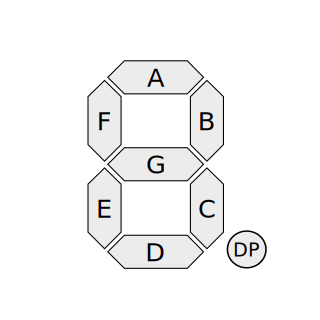
\includegraphics[height=3cm]{pictures/7segdetails.pdf}}
	\caption{Détail et Annotation d'un 7 segment par \href{https://commons.wikimedia.org/wiki/User:H2g2bob}{H2g2bob} - \ccLogo\ccAttribution\ccShareAlike}
\end{figure}

\begin{table}[H]
\centering
\begin{tabular}{|c|c|c|c|c|c|c|c|}
	\hline
		& \multicolumn{7}{c|}{Individual Segments} \\
	\hline
	Display & A & B & C & D & E & F & G \\
	\hline
	0       & 1 & 1 & 1 & 1 & 1 & 1 & 0 \\
	\hline
	1       & 0 & 1 & 1 & 0 & 0 & 0 & 0 \\
	\hline
	2       & 1 & 1 & 0 & 1 & 1 & 0 & 1 \\
	\hline
	3       & 1 & 1 & 1 & 1 & 0 & 0 & 1 \\
	\hline
	4       & 0 & 1 & 1 & 0 & 0 & 1 & 1 \\
	\hline
	5       & 1 & 0 & 1 & 1 & 0 & 1 & 1 \\
	\hline
	6       & 1 & 0 & 1 & 1 & 1 & 1 & 1 \\
	\hline
	7       & 1 & 1 & 1 & 0 & 0 & 0 & 0 \\
	\hline
	8       & 1 & 1 & 1 & 1 & 1 & 1 & 1 \\
	\hline
	9       & 1 & 1 & 1 & 1 & 0 & 1 & 1 \\
	\hline
	A       & 1 & 1 & 1 & 0 & 1 & 1 & 1 \\
	\hline
	B       & 0 & 0 & 1 & 1 & 1 & 1 & 1 \\
	\hline
	C       & 1 & 0 & 0 & 1 & 1 & 1 & 0 \\
	\hline
	D       & 0 & 1 & 1 & 1 & 1 & 0 & 1 \\
	\hline
	E       & 1 & 0 & 0 & 1 & 1 & 1 & 1 \\
	\hline
	F       & 1 & 0 & 0 & 0 & 1 & 1 & 1 \\
	\hline
\end{tabular}
	\caption{Décomposition des caractères hexadécimaux en segments}
\end{table}

\subsection{Mise en place sur logisim}
\paragraph{}
La table de vérité présentée dans la section précèdente peut être utilisée pour obtenir une fonction simplifiée de chaque segment en utilisant les tables de Karnaugh\footnote{\url{https://fr.wikipedia.org/wiki/Table_de_Karnaugh}}. Logisim embarque une fonctionnalité permettant d'effectuer cette analyse de manière simplifiée. Pour celà il est nécessaire de lancer logisim avec l'option -analyze soit dans notre cas :

\begin{lstlisting}[language=bash]
java -jar logisim-evolution.jar -analyze
\end{lstlisting}

\paragraph{}
En utilisant ce paramètre une option apparaît dans le menu "Projet"->"Analyser le circuit". Il est possible dans l'onglet "table" de remplir la table de vérité du circuit. Une fois le tableau complété, cliquer sur "Construire le circuit" générera le circuit correspondant. Ce dernier devrait ressembler à ceci :
\begin{figure}[H]
        \makebox[\textwidth]{\includegraphics[width=4cm]{pictures/sevendecoder.png}}
	\caption{Contenu du composant "Seven segment decoder"}
\end{figure}



\section{ALU}

\subsection{Description}

	L'unité arithmétique et logique est l'élèment qui se charge des calculs au sein du processeur. Les ALU les plus basiques ne font que des opérations sur des entiers cependant on trouve des ALU spécialisées. Les calculs sur ces dernières vont des opérations à virgule flottante jusqu'à des calculs plus complexes tels que des racines carrées, des logarithmes, des sinus ou cosinus... Notre ALU n'effectuera que des calculs simples (addition, soustraction, multiplication, décalage) sur des entiers de 32 bits.

	Une ALU comporte deux entrées amenant les données à traiter. Une troisième entrée permet de désigner le calcul à effectuer. En sortie on retrouvera le résultat de l'opération ainsi que des drapeaux. Ces drapeaux représentent une série d'état à la suite d'un calcul : un résultat négatif, un résultat nul, un débordement ou encore une retenue. 

L'entrée \texttt{Shift} indique le nombre de décalage pour les opérations de décalage.


\paragraph{Remarque:} les instructions \texttt{TST}, \texttt{CMP}, \texttt{CMN} n'enregistrent pas le résultat de l'opération. Seuls les drapeaux sont mis à jour.
Pour ces opérations en particulier, il faudra recopier l'entrée \texttt{B} sur la sortie \texttt{S}. Le contrôleur définiera le même registre pour le registre \texttt{Rn} d'opérande B que pour le registre \texttt{Rd} de destination de la sortie S.

\paragraph{Remarque 2:} pour l'instruction \texttt{SBC}, la retenue entrante doit être inversée (voir \textit{\ref{subsubsubsec:SBC}~\nameref{subsubsubsec:SBC}}).

\subsection{Interface}

\subsubsection{Entrées}

\begin{tabular}{|l|r|l|}
\hline
\textbf{Port}		& \textbf{Taille} & \textbf{Description}\\
\hline

\texttt{A}		& \texttt{32} & Première opérande\\
\hline
\texttt{B}		& \texttt{32} & Seconde opérande\\
\hline
\texttt{Shift}		&  \texttt{5} & Nombre de décalage\\
\hline
\texttt{CarryIn}	&  \texttt{1} & Retenu entrente\\
\hline
\texttt{Codop}		&  \texttt{4} & Code opération ALU\\

\hline
\end{tabular}


\subsubsection{Sorties}

\begin{tabular}{|l|r|l|}
\hline 
\textbf{Port} & \textbf{Taille} & \textbf{Description}\\
\hline

\texttt{S}	& \texttt{32} & Registre résultat\\
\hline
\texttt{Flags}	&  \texttt{4} & Registre drapeaux, ordre: \texttt{NZCV}\\

\hline
\end{tabular}


\subsection{Opérations}
\label{subsec:Opcodes}
Ces opérations de l'ALU correspondent exactement aux instructions de la catégorie \textit{Data Processing}. En cas de doute, se référer à \textit{\ref{sec:ISA}~\nameref{sec:ISA}}.

\begin{tabular}{|r|c|l|l|}
\hline
\textbf{Codop}  & \textbf{Opération}	& \textbf{Instructions} & \textbf{Remarque}\\
\hline

$0000$ & \texttt{A and B}			& AND			&\\
\hline
$0001$ & \texttt{A xor B}			& EOR			&\\
\hline
$0010$ & \texttt{B << Shift}			& LSL			& Retenue sortante, voir jeu d'instruction\\
\hline
$0011$ & \texttt{B >> Shift}			& LSR			& Retenue sortante, voir jeu d'instruction\\
\hline
$0100$ & \texttt{B >> Shift (arith)}		& ASR			& Retenue sortante, voir jeu d'instruction\\
\hline
$0101$ & \texttt{A + B + CarryIn}		& ADC			&\\
\hline
$0110$ & \texttt{A – B + CarryIn – 1}		& SBC			& Retenue entrante inversée\\
\hline
$0111$ & \texttt{B >> Shift (rot)}		& ROR			& Retenue sortante, voir jeu d'instruction\\
\hline
$1000$ & \texttt{A and B}			& TST			& Résultat perdu, seuls les drapeaux sont mis à jour\\
\hline
$1001$ & \texttt{0 – A}				& RSB			& Registre Rm utilisé plutôt que Rn\\
\hline
$1010$ & \texttt{A – B}				& CMP			& Résultat perdu, seuls les drapeaux sont mis à jour\\
\hline
$1011$ & \texttt{A + B}				& CMN			& Résultat perdu, seuls les drapeaux sont mis à jour\\
\hline
$1100$ & \texttt{A or B}			& ORR			&\\
\hline
$1101$ & \texttt{A * B}				& MUL			&\\
\hline
$1110$ & \texttt{A and not B}			& BIC			&\\
\hline
$1111$ & \texttt{Not B}				& MVN			&\\
\hline
\end{tabular}

\subsection{Drapeaux}

Ces drapeaux de l'ALU correspondent exactement aux drapeaux de l'architecture ARM. En cas de doute, se référer à \textit{\ref{sec:ISA}~\nameref{sec:ISA}} et \textit{\ref{subsec:Flags}~\nameref{subsec:Flags}} .

\begin{tabular}{|c|l|l|}
\hline
\textbf{Symbole} & \textbf{Nom} & \textbf{Description}\\
\hline

\texttt{N}	& \texttt{Negative}	& Résultat négatif\\
\hline
\texttt{Z}	& \texttt{Zero}		& Résultat nul\\
\hline
\texttt{C}	& \texttt{CarryOut}	& Retenue sortante (dépassement de capacité non-signé)\\
\hline
\texttt{V}	&  \texttt{Overflow}	& Dépassement de capacité signé\\

\hline
\end{tabular}

\section{Banc de registres}

\subsection{Description}

\subsection{Interface}

\subsubsection{Entrées}

\begin{tabular}{|l|r|l|}
\hline
\textbf{Port}		& \textbf{Taille} & \textbf{Description}\\
\hline

\texttt{DataIn}		& \texttt{32} & Données entrantes, à enregistrer dans le registre sélectionné\\
\hline
\texttt{RegDest}	&  \texttt{3} & Sélection du registre de destination des données entrantes\\
\hline
\texttt{Clk}		&  \texttt{1} & Horloge\\
\hline
\texttt{Reset}		&  \texttt{1} & Remise à zéro\\
\hline
\texttt{RegA}		&  \texttt{3} & Sélection du registre A pour les données sortantes\\
\hline
\texttt{RegB}		&  \texttt{3} & Sélection du registre B pour les données sortantes\\

\hline
\end{tabular}


\subsubsection{Sorties}

\begin{tabular}{|l|r|l|}
\hline 
\textbf{Port} & \textbf{Taille} & \textbf{Description}\\
\hline

\texttt{AOut}	& \texttt{32} & Données sortantes du registre sélectionné A\\
\hline
\texttt{BOut}	& \texttt{32} & Données sortantes du registre sélectionné B\\
\hline
\texttt{R0}	& \texttt{32} & Registre interne 0\\
\hline
\texttt{R1}	& \texttt{32} & Registre interne 1\\
\hline
\texttt{R2}	& \texttt{32} & Registre interne 2\\
\hline
\texttt{R3}	& \texttt{32} & Registre interne 3\\
\hline
\texttt{R4}	& \texttt{32} & Registre interne 4\\
\hline
\texttt{R5}	& \texttt{32} & Registre interne 5\\
\hline
\texttt{R6}	& \texttt{32} & Registre interne 6\\
\hline
\texttt{R7}	& \texttt{32} & Registre interne 7\\

\hline
\end{tabular}

Les sorties \texttt{R0-R7} ne seront pas utilisées pour implémenter une quelconque fonctionalité. Elles sont présentes pour aider à visualiser le comportement du processeur.

\subsection{Interaction avec l'ALU}

Après avoir réalisé l'ALU et le banc de registres, l'interaction entre ces composants peut être mise en oeuvre de la manière suivante:

\hspace{14em}
\includegraphics[scale=0.5]{pictures/ALU_Registers.pdf}

Il est ainsi possible de valider leur comportement en enregistrant des données dans le banc de registre (à l'aide des ports \texttt{DataIn} et \texttt{RegDest})
puis en effectuant diverses opération par l'ALU en spécifiant  le \texttt{Codop}.

\section{Usage de la documentation ARM} 
\subsection{nyan} 
\subsubsection{meow} 
\subsubsubsection{mjau} 
miaounyanmeowmjau


\end{document}
